\documentclass[a4j,12pt,]{jarticle}
 \usepackage[dvipdfmx]{graphicx}
 \usepackage{float}
 \usepackage{siunitx} %%SI単位系用
 \usepackage{amssymb, amsmath}
 \usepackage{ascmac,here,txfonts,txfonts}
\usepackage{listings,jlisting}
\usepackage[dvipdfmx]{color}
\lstset{%
  language={Python},
  basicstyle={\small},%
  identifierstyle={\small},%
  commentstyle={\small\itshape\color[rgb]{0,0.5,0}},%
  keywordstyle={\small\bfseries\color[rgb]{0,0,1}},%
  ndkeywordstyle={\small},%
  stringstyle={\small\ttfamily\color[rgb]{1,0,1}},
  frame={tb},
  breaklines=true,
  columns=[l]{fullflexible},%
  numbers=left,%
  xrightmargin=0zw,%
  xleftmargin=3zw,%
  numberstyle={\scriptsize},%
  stepnumber=1,
  numbersep=1zw,%
  lineskip=-0.5ex%
}
\begin{document}

{\noindent\small 第6回報告書 \hfill\today}
\begin{center}
  {\Large 相互コレログラムを用いた日射量の日時推定誤差の減少}
\end{center}
\begin{flushright}
  祖父江匠真 \\
\end{flushright}

\section{はじめに}
前回, リサイクル館から送信された太陽光発電の日射量データと, 計算によって求めた日射量との間の, 日時推定の誤差の大きさを求めることで評価した.
しかし, 日時誤差が最小になるような時間シフトを行っていなかったので、今回は相互コレログラムを用いて日時誤差が最小になるラグの選定と, 選定したラグを加えた上で日時誤差を求めて評価を行った.

\section{相互コレログラムによる最小ラグの選定}
実測値の時系列データの範囲を2022年5月21日0時0分から2022年5月28日12時0分までの7.5日間として, 計算値の時系列データの範囲を2022年5月20日18時0分から2022年5月27日18時0分までの7日間とする.
相互コレログラムは, 計算値の時系列データを最大で12時間(0.5日)シフトするようなラグを与え, ラグごとに計測値と, シフトした計算値の時系列データと対応する実測値部分との内積を求めることで相互相関を計算する.
その際, 相互相関の最大値を取るラグを最小ラグとして採用する.
% また, 実測値と計算値の間で時系列データの範囲を0.25日(6時間)ずらしているので, 相互相関は相互コレログラムの中心付近で最大値を取ると推測される.

図\ref{p1}に, 上記の条件で計算した相互コレログラムを示す.
図\ref{p1}から, 実測値と計算値を809秒ずらすことで相互相関の値が最大となることが分かった.

\begin{figure}[H]
  \begin{center}
    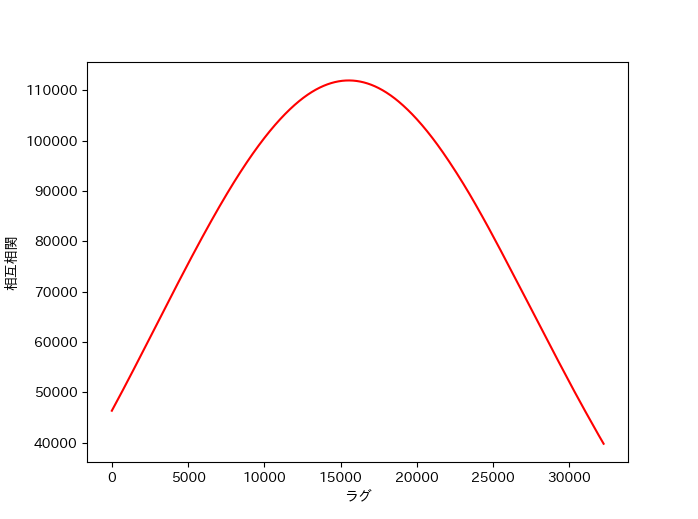
\includegraphics[width=160mm]{correlogram.png}
    \caption{相互コレログラム}
    \label{p1}
  \end{center}
\end{figure}

\section{相互コレログラムから得られたラグ用いた日時誤差による評価}
評価するに当たり, Elasticsearchサーバーから取得した2022年5月21日の日射量データと, リサイクル館の緯度経度と日付情報(2022年5月21日)を入力として求めた日射量の計算値を使用する.

日射量の計算式を用いて日時を予測した際の日時誤差を, ある日時について求めた計算値と同じ日射量を取る実測値の日時との日時差を計算することで求める.

図\ref{p2}に, ラグを加えずに計算した日射量と実測値との日時誤差のグラフを示す.
図\ref{p2}から, ラグを加えずに計算した日射量による日時推定には最大で約60分の誤差が生じることが分かった.

\begin{figure}[H]
  \begin{center}
    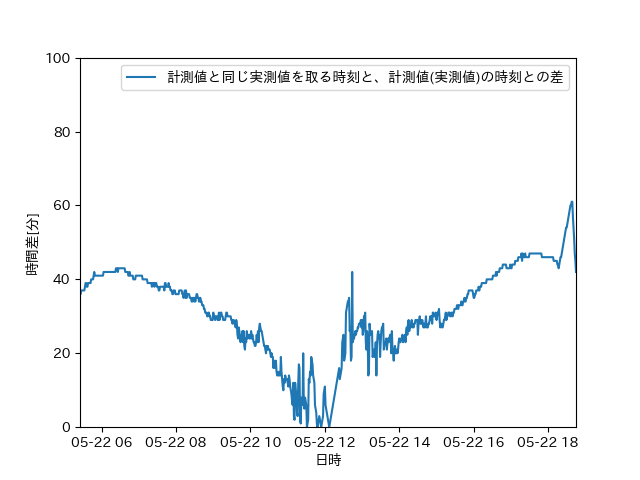
\includegraphics[width=160mm]{dt_diff.png}
    \caption{計測値と同じ実測値を取る日時と、計測値の日時との差(ラグなし)}
    \label{p2}
  \end{center}
\end{figure}

次に, 相互コレログラムから得られたラグを加えて計算した日射量と実測値との日時誤差のグラフを図\ref{p3}に示す.
図\ref{p2}, 図\ref{p3}より, ラグを加えることで日時誤差の最大値が60分から56分に減少した.

\begin{figure}[H]
  \begin{center}
    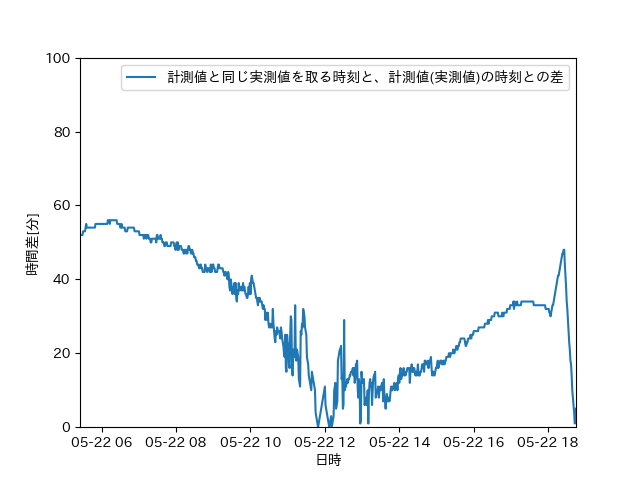
\includegraphics[width=160mm]{dt_diff_with_delay.png}
    \caption{計測値と同じ実測値を取る日時と、計測値の日時との差(ラグあり)}
    \label{p3}
  \end{center}
\end{figure}

\section{おわりに}
今回は相互コレログラムを用いて相互相関が最大となるラグの選定, 選定したラグを用いて実測値と計算値の日時誤差を求めることで評価した.

相互コレログラムから得られたラグを加えることで日時誤差の最大値が60分から56分に減少した.
% 相互コレログラムを用いた日時誤差の減少には大きな効果が得られなかったので, 次は日射量の計算式を再検討する.

\begin{thebibliography}{5}
  \bibitem{1}mattip, "numpy/numeric.py at v1.22.4 · numpy/numpy",\\ "https://github.com/numpy/numpy/blob/v1.22.4/numpy/core/numeric.py\#L670-L741", 参照 June 6, 2022.
\end{thebibliography}

\end{document}